\documentclass[aspectratio=169,dvipsnames]{beamer}

\usetheme{femto}

\usepackage[english]{babel}
\usepackage[T1]{fontenc}
\usepackage{xcolor}
\usepackage{adjustbox}
\usepackage{multirow}
\usepackage{nicematrix}
\usepackage{url}
\usepackage{amsmath, amssymb}

%
% Enables marks.
\usepackage{pifont}
\newcommand{\cmark}{\color{ForestGreen}{\ding{51}}}
\newcommand{\xmark}{\color{red}{\ding{55}}}

%
% Imports tikz and its used libraries.
\usepackage{tikz}
\usetikzlibrary{shapes.arrows}
\usetikzlibrary{pgfplots.groupplots}

%
% Imports libraries for reading csv files and turning them into figures.
\usepackage{pgfplots}
\usepackage{pgfplotstable}
\pgfplotsset{compat=1.18}

%
% Import the csv files used to build the results figures on the synthetic datasets.
\pgfplotstableread[col sep=comma]{./figures/data/IQR_synthetics_results.csv}\IQRResultsSynthetics
\pgfplotstableread[col sep=comma]{./figures/data/Hino_synthetics_results.csv}\HinoResultsSynthetics
\pgfplotstableread[col sep=comma]{./figures/data/IF_synthetics_results.csv}\IFResultsSynthetics
\pgfplotstableread[col sep=comma]{./figures/data/SVM_synthetics_results.csv}\SVMResultsSynthetics
\pgfplotstableread[col sep=comma]{./figures/data/LOF_synthetics_results.csv}\LOFResultsSynthetics

%
% Defines global tikz styles for :
% - blue arrows;
% - the ability to hide or show content for slides 
\tikzset{%
	arrowstyle/.style n args=3{%
	single arrow,
	fill=femtogreenstrong,
	anchor=base,
	align=center,
	minimum height=#1,
	single arrow head extend=#2,
	inner sep=#3
	},
	invisible/.style={opacity=0},
	visible on/.style={alt={#1{}{invisible}}},
	alt/.code args={<#1>#2#3}{%
	\alt<#1>{\pgfkeysalso{#2}}{\pgfkeysalso{#3}} % \pgfkeysalso doesn't change the path
	}
}
\newcommand{\tikzarrow}[3]{%
	\tikz[baseline=-0.5ex]\node[arrowstyle={#1}{#2}{#3}] {};
}

%
% Gaussian function useful for IQR figure
\usepgfplotslibrary{fillbetween}
\pgfmathdeclarefunction{gauss}{3}{%
  \pgfmathparse{1/(#3*sqrt(2*pi))*exp(-((#1-#2)^2)/(2*#3^2))}%
}


%
% Presentation information.
\title{Hunting Inside N-Quantiles of Outliers (Hino)}
\subtitle{The 29th Pacific-Asia Conference on Knowledge Discovery and Data Mining}
\author[Jessy COLONVAL]{\textbf{Jessy COLONVAL\inst{1}} and Fabrice BOUQUET\inst{1}}
\institute{%
	\inst{1} FEMTO-ST Institute, CNRS, Univ. Marie \& Louis Pasteur (MLP), Besançon, France
}
\date{13 June 2025}


\begin{document}

\begin{frame}[plain, c]
	\titlepage
\end{frame}

\begin{frame}{What is an outlier?}
	This is a point that is inconsistent with the rest of the dataset.
	\vspace{0.25cm}

	Inconsistence have two effects on ML:
	\begin{itemize}
		\item In learning phase: Weaken the predictive power.
		\item In validation phase: Weaken the cross-validation score.
	\end{itemize}
	\vspace{0.25cm}

	They must therefore be removed from corpus
	\vspace{0.5cm}

	\textbf{Research questions:}
	\begin{enumerate}
		\item How do you characterize an outlier?
		\item It's possible to have an automatic method?
	\end{enumerate}
	\tikzarrow{0.75cm}{0.15cm}{0.1cm}Validation on real and synthetic datasets
\end{frame}

\begin{frame}{How we define outliers}
	\begin{minipage}[t]{0.64\linewidth}
		\begin{figure}
			\centering
			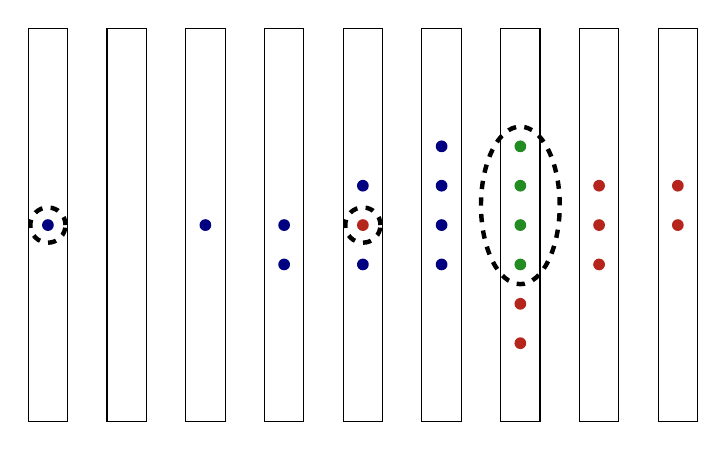
\begin{tikzpicture}
				\draw[draw=black, visible on=<1->] (-4,0) rectangle ++(0.5,5);
				\draw[draw=black, visible on=<1->] (-3,0) rectangle ++(0.5,5);
				\draw[draw=black, visible on=<1->] (-2,0) rectangle ++(0.5,5);
				\draw[draw=black, visible on=<1->] (-1,0) rectangle ++(0.5,5);
				\draw[draw=black, visible on=<1->] (0,0) rectangle ++(0.5,5);
				\draw[draw=black, visible on=<1->] (1,0) rectangle ++(0.5,5);
				\draw[draw=black, visible on=<1->] (2,0) rectangle ++(0.5,5);
				\draw[draw=black, visible on=<1->] (3,0) rectangle ++(0.5,5);
				\draw[draw=black, visible on=<1->] (4,0) rectangle ++(0.5,5);

				% Points outliers
				\node[visible on=<1->] at (-3.75,2.5) [circle, fill=NavyBlue, inner sep=1.5pt] {};
				\node[draw, dashed, ultra thick, visible on=<2>] at (-3.75,2.5) [circle, black, inner sep=4.5pt] {};

				% All class in one quantile.
				\node[visible on=<1->] at (2.25,1.5) [circle, fill=BrickRed, inner sep=1.5pt] {};
				\node[visible on=<1->] at (2.25,3.5) [circle, fill=ForestGreen, inner sep=1.5pt] {};
				\node[visible on=<1->] at (2.25,3.0) [circle, fill=ForestGreen, inner sep=1.5pt] {};
				\node[visible on=<1->] at (2.25,2.0) [circle, fill=ForestGreen, inner sep=1.5pt] {};
				\node[visible on=<1->] at (2.25,2.5) [circle, fill=ForestGreen, inner sep=1.5pt] {};
				\node[visible on=<1->] at (2.25,1.0) [circle, fill=BrickRed, inner sep=1.5pt] {};
				\draw[dashed, ultra thick, visible on=<4>] (2.25,2.75) ellipse (0.5cm and 1cm);

				% Q2
				\node[visible on=<1->] at (-1.75, 2.5) [circle, fill=NavyBlue, inner sep=1.5pt] {};

				% Q3
				\node[visible on=<1->] at (-0.75, 2.5) [circle, fill=NavyBlue, inner sep=1.5pt] {};
				\node[visible on=<1->] at (-0.75, 2.0) [circle, fill=NavyBlue, inner sep=1.5pt] {};

				% Q4.
				\node[visible on=<1->] at (0.25, 2.5) [circle, fill=BrickRed, inner sep=1.5pt] {};
				\node[visible on=<1->] at (0.25, 3) [circle, fill=NavyBlue, inner sep=1.5pt] {};
				\node[visible on=<1->] at (0.25, 2.0) [circle, fill=NavyBlue, inner sep=1.5pt] {};
				\node[draw, dashed, ultra thick, visible on=<3>] at (0.25, 2.5) [circle, black, inner sep=4.5pt] {};

				% Q5.
				\node[visible on=<1->] at (1.25, 2.5) [circle, fill=NavyBlue, inner sep=1.5pt] {};
				\node[visible on=<1->] at (1.25, 2) [circle, fill=NavyBlue, inner sep=1.5pt] {};
				\node[visible on=<1->] at (1.25, 3) [circle, fill=NavyBlue, inner sep=1.5pt] {};
				\node[visible on=<1->] at (1.25, 3.5) [circle, fill=NavyBlue, inner sep=1.5pt] {};

				% Q6
				\node[visible on=<1->] at (3.25, 3) [circle, fill=BrickRed, inner sep=1.5pt] {};
				\node[visible on=<1->] at (3.25, 2.5) [circle, fill=BrickRed, inner sep=1.5pt] {};
				\node[visible on=<1->] at (3.25, 2) [circle, fill=BrickRed, inner sep=1.5pt] {};

				% Q7
				\node[visible on=<1->] at (4.25, 2.5) [circle, fill=BrickRed, inner sep=1.5pt] {};
				\node[visible on=<1->] at (4.25, 3.0) [circle, fill=BrickRed, inner sep=1.5pt] {};
			\end{tikzpicture}
		\end{figure}
	\end{minipage}
	\hfill
	\begin{minipage}[t]{0.35\linewidth}
		\textbf{Quantiles must be:}
		\begin{itemize}
			\item small enough to have close points;
			\item large enough to contain one per class.
		\end{itemize}
		Number of quantile is $\frac{n_{p}}{n_{c} + 1}$.
		\vspace{0.25cm}

		\pause
		\textbf{Isolation of a point:}
		\begin{itemize}
			\item In space.
			\pause
			\item From its peers.
		\end{itemize}
		\vspace{0.25cm}

		\pause
		Can't be isolated if all points of a class are in one quantile.
	\end{minipage}
\end{frame}

\begin{frame}{Hino's algorithm}
	Is an extension of the \textbf{IQR} method.
	\vspace{0.25cm}

	\textbf{Isolation tolerance:}
	\begin{itemize}
		\item Being isolated doesn't necessarily mean being an outlier;
		\item A point can be isolated in several attributes.
	\end{itemize}
	\tikzarrow{0.75cm}{0.15cm}{0.1cm}Establish an isolation tolerance before a point is considered an outlier.
	\vspace{0.25cm}

	\textbf{How it works:}
	\begin{itemize}
		\item Splits points into several quantiles for each attribute;
		\item \textbf{Isolation score of a point}: number of times is in a quantile where its class isn't present in the $2$ adjacent ones;
		\item \textbf{Outlier}: isolation score $\geq$ tolerance limit;
		\item Restarts with tolerance limit $+1$ if: \% outlier detected $>$ the \% allowed.
	\end{itemize}
\end{frame}

\begin{frame}{Objectives of experiments}
	\textbf{Determine if Hino is:}
	\begin{itemize}
	\item A \textcolor{ForestGreen}{\textbf{viable}} method:
	\begin{itemize}
		\item Removes a maximum of outliers.
		\item Don't removes too much healthy points.
		\item Doesn't eliminate a class.
	\end{itemize}
	\item \textcolor{ForestGreen}{\textbf{Better}} than the state-of-the-art methods:\\ IQR [15], SVM [2], Isolation Forest [12] and LOF [4].
	\end{itemize}
	\vspace{0.25cm}

	\textbf{The evaluation was realized on:}\\
	\vspace{0.25cm}
	\begin{minipage}[c]{0.39\linewidth}
	\begin{itemize}
		\item \textcolor{ForestGreen}{$\mathbf{278}$} synthetic datasets:
		\begin{itemize}
		\item Large amount of sample.
		\item Outliers are known.
		\item Bias i.r. of real world.
		\end{itemize}
	\end{itemize}
	\end{minipage}
	\hfill
	\begin{minipage}[c]{0.6\linewidth}
	\begin{itemize}
		\item \textcolor{ForestGreen}{$\mathbf{16}$} real datasets:
		\begin{itemize}
		\item Representative i.r. characteristics.
		\item Outliers are unknown.
		\item Real usage.
		\end{itemize}
	\end{itemize}
	\end{minipage}
\end{frame}

\begin{frame}{Synthetic datasets}
	\textbf{How they created:}
	\begin{itemize}
	\item Generate with the algorithm used to create Madelon (from UCI) [8].
	\item Modify $5$\% of points and make them outliers:
	\begin{itemize}
		\item Preserve representativity of dataset.
		\item Choose points with unanimity predicted by ML.
		\item Change randomly their classes.
	\end{itemize}
	\end{itemize}
	\vspace{0.5cm}

	\begin{minipage}[c]{0.49\linewidth}
	\textbf{Two kinds of measure:}
	\begin{itemize}
		\item \textcolor{BrickRed}{\textbf{Sensitivity}} \tikzarrow{0.75cm}{0.15cm}{0.1cm}\% correctly predicted outliers
		\item \textcolor{ForestGreen}{\textbf{Specificity}} \tikzarrow{0.75cm}{0.15cm}{0.1cm}\% correctly predicted healthy points.
	\end{itemize}
	\end{minipage}
	\hfill
	\begin{minipage}[c]{0.49\linewidth}
	\begin{adjustbox}{max width=\textwidth}
		\centering
		\begin{tabular}{|l|l|l|}
		\hline
		\textbf{Samples} & \textbf{Attributes} & \textbf{Classes} \\
		\hline
		$250$ & $10 \ldots 50, 25$ & $2 \ldots 5$ \\
		$500$ & $10 \ldots 70, 25, 75$ & $2 \ldots 5$ \\
		$1\,000$ & $10 \ldots 100, 25, 75$ & $2 \ldots 7$ \\
		$2\,500$ & $10 \ldots 100, 25, 75$ & $2 \ldots 8$ \\
		$5\,000$ & $10 \ldots 100, 25, 75, 125$ & $2 \ldots 11$ \\
		\hline
		\end{tabular}
	\end{adjustbox}
	\end{minipage}
\end{frame}

\begin{frame}{Synthetic Results}
	\begin{adjustbox}{max height=0.8\textheight, center}
	\begin{tikzpicture}
		\pgfplotsset{every tick label/.append style={font=\Large}}
		
		\begin{groupplot}[%
			group style = {group size = 3 by 2, horizontal sep = 60pt, vertical sep = 60pt}
		]
		\nextgroupplot[%
			title={\Huge\textbf{IQR}},
			ylabel={\LARGE\textcolor{BrickRed}{\textbf{sensitivity}}},
			ymin=0, ymax=100,
			grid
		]
			\addplot[only marks, mark size=0.8] table  [x={specificity}, y={sensitivity}] {\IQRResultsSynthetics};
	
		\nextgroupplot[%
			title={\Huge\textbf{Isolation Forest}},
			xlabel={\LARGE\textcolor{ForestGreen}{\textbf{specificity}}},
			ymin=0, ymax=100,
			grid
		]
			\addplot[only marks, mark size=0.8] table  [x={specificity}, y={sensitivity}] {\IFResultsSynthetics};
	
		\nextgroupplot[%
			title={\Huge\textbf{SVM}},
			ymin=0, ymax=20,
			grid
		]
			\addplot[only marks, mark size=0.8] table  [x={specificity}, y={sensitivity}] {\SVMResultsSynthetics};
	
		\nextgroupplot[%
			title={\Huge\textbf{LOF}},
			ylabel={\LARGE\textcolor{BrickRed}{\textbf{sensitivity}}},
			ymin=0, ymax=20,
			grid
		]
			\addplot[only marks, mark size=0.8] table  [x={specificity}, y={sensitivity}] {\LOFResultsSynthetics};
	
		\nextgroupplot[group/empty plot,]

		\nextgroupplot[%
			title={\Huge\textbf{Hino}},
			ymin=0, ymax=100,
			grid
		]
			\addplot[only marks, mark size=0.8] table  [x={specificity}, y={sensitivity}] {\HinoResultsSynthetics};
		\end{groupplot}
	\end{tikzpicture}
	\end{adjustbox}
\end{frame}

\begin{frame}{Real datasets}
	\begin{minipage}[c]{0.46\linewidth}
	\textbf{UCI Machine Learning Repository:}
	\begin{itemize}
		\item Classification.
		\item Continuous values.
		\item Cover several combination of characteristics.
	\end{itemize}
	\end{minipage}
	\hfill
	\begin{minipage}[c]{0.53\linewidth}
	\begin{tikzpicture}[scale=0.9]
		\node[text width=\textwidth] at (0, 0) {\textbf{Two kinds of measures (with 6 ML):}};

		\node[text width=\textwidth] at (0.25, -0.5) {\textcolor{femtogreenstrong}{$\blacktriangleright$}~~Cross-validation:};
		\node[text width=5.25cm] (A) at (-0.4,-1.0) {\textcolor{femtogreenstrong}{\small$\blacktriangleright$}~~Detected outliers removed.};
		\node[text width=5.25cm] (B) at (-0.4,-1.5) {\textcolor{femtogreenstrong}{\small$\blacktriangleright$}~~$70$\% train + $30$\% test};
		\node[text width=5.25cm] (C) at (-0.4, -2.0) {\small\tikzarrow{0.75cm}{0.15cm}{0.1cm}\% good prediction.};

		\node[text width=\textwidth] at (0.25, -2.5) {\textcolor{femtogreenstrong}{\small$\blacktriangleright$}~~False positivity:};
		\node[text width=6.5cm] (D) at (0.295,-3.0) {\textcolor{femtogreenstrong}{\small$\blacktriangleright$}~~Healthy as train \& Outliers as test.};
		\node[text width=6.5cm] (E) at (0.295,-3.5) {\small\tikzarrow{0.75cm}{0.15cm}{0.1cm}\% good prediction.};

		\draw[<->, bend left=-45, thick, femtopurplestrong] (C.east) to node[midway, right] {\small x10} (A.east);
		\draw[<->, bend left=-45, thick, femtopurplestrong] (E.east) to node[midway, right] {\small x10} (D.east);
	\end{tikzpicture}
	\end{minipage}
	\vspace{0.25cm}

	\begin{adjustbox}{max height=0.2\textheight,center}
	\begin{tabular}{|l|c|c|c|}
		\hline
		\textbf{Datasets} & \textbf{Points} & \textbf{Attributes} & \textbf{Classes} \\
		\hline
		annthyroid & $7\,200$ & $21$ & $3$ \\
		breastW & $683$ & $9$ & $2$ \\
		cardio & $2\,126$ & $21$ & $10$ \\
		glass & $214$ & $9$ & $6$ \\
		ionosphere & $351$ & $33$ & $2$ \\
		isolet & $7\,797$ & $617$ & $26$ \\
		letter & \multirow{2}{*}{$20\,000$} & \multirow{2}{*}{$16$} & \multirow{2}{*}{$26$} \\
		recognition & & & \\
		mammo\- & \multirow{2}{*}{$11\,183$} & \multirow{2}{*}{$6$} & \multirow{2}{*}{$2$} \\
		graphy & & & \\
		\hline
	\end{tabular}
	\hspace{0.25cm}
	\begin{tabular}{|l|c|c|c|}
		\hline
		\textbf{Datasets} & \textbf{Points} & \textbf{Attributes} & \textbf{Classes} \\
		\hline
		multiple & \multirow{2}{*}{$2\,000$} & \multirow{2}{*}{$619$} & \multirow{2}{*}{$10$} \\
		features & & & \\
		musk & $6\,598$ & $166$ & $2$ \\
		parkinson & $756$ & $752$ & $2$ \\
		pendigits & $10\,992$ & $16$ & $10$ \\
		satimage2 & $6\,435$ & $36$ & $6$ \\
		shuttle & $58\,000$ & $9$ & $7$ \\
		wine & $178$ & $13$ & $3$ \\
		wine\- & \multirow{2}{*}{$1\,599$} & \multirow{2}{*}{$11$} & \multirow{2}{*}{$6$} \\
		quality & & & \\
		\hline
	\end{tabular}
	\end{adjustbox}
\end{frame}

\begin{frame}{Example results on real datasets}
	\begin{minipage}[c]{0.45\linewidth}
	Generally, Hino:
	\begin{itemize}
		\item \small \textcolor{BlueViolet}{Removes less points.}
		\item \small \textcolor{ForestGreen}{Gives a better cross-validation.}
		\item \small \textcolor{Orange}{Gives a better false-positivity.}
		\item \small \textcolor{Purple}{Tolerance limit calculated is relevant.}
	\end{itemize}
	\end{minipage}
	\hfill
	\begin{minipage}[c]{0.54\linewidth}
	Over $16$ real datasets:
	\begin{itemize}
		\item $13$ gives \textbf{Hino} as better solution.
		\item $2$ is even between \textbf{Hino} and \textbf{LOF}.
		\item $1$ is even between \textbf{Hino}, \textbf{LOF} and \textbf{SVM}.
	\end{itemize}
	\end{minipage}
	\vspace{0.25cm}

	\begin{adjustbox}{max width=\textwidth}
	\begin{NiceTabular}{lcccccccccccc}
	\CodeBefore
		% cardio
		\cellcolor{gray!40}{4-12}
		\cellcolor{gray!40}{5-12}
		\cellcolor{gray!40}{6-12}
		\cellcolor{gray!40}{4-13}
		\cellcolor{gray!40}{5-13}
		\cellcolor{gray!40}{6-13}
		% pendigits
		\cellcolor{gray!40}{7-12}
		\cellcolor{gray!40}{8-12}
		\cellcolor{gray!40}{9-12}
		\cellcolor{gray!40}{7-13}
		\cellcolor{gray!40}{8-13}
		\cellcolor{gray!40}{9-13}
	\Body
	& \Block{1-2}{\textbf{IQR}} & & \Block{1-2}{\textbf{Isolation Forest}} & & \Block{1-2}{\textbf{SVM}} & & \Block{1-2}{\textbf{LOF}} & & \Block{1-2}{\textbf{Hino}} & & \Block{1-2}{\textbf{Best of Hino}} & \\
	\Block{2-1}{\textbf{Datasets}} & \textbf{Cross} & \textbf{False} & \textbf{Cross} & \textbf{False} & \textbf{Cross} & \textbf{False} & \textbf{Cross} & \textbf{False} & \textbf{Cross} & \textbf{False} & \textbf{Cross} & \textbf{False} \\
	& \textbf{validation} & \textbf{positive} & \textbf{validation} & \textbf{positive} & \textbf{validation} & \textbf{positive} & \textbf{validation} & \textbf{positive} & \textbf{validation} & \textbf{positive} & \textbf{validation} & \textbf{positive} \\

	% cardio
	\Block{3-1}{cardio} & \textcolor{ForestGreen}{$81.40\%$} & \textcolor{Orange}{$60.35\%$} & \textcolor{ForestGreen}{$81.23\%$} & \textcolor{Orange}{$72.71\%$} & \textcolor{ForestGreen}{$82.06\%$} & \textcolor{Orange}{$71.67\%$} & \textcolor{ForestGreen}{$82.45\%$} & \textcolor{Orange}{$71.67\%$} & \textcolor{ForestGreen}{$83.16\%$} & \textcolor{Orange}{$39.72\%$} & \textcolor{ForestGreen}{$84.76\%$} & \textcolor{Orange}{$43.77\%$} \\
	& $\pm1.94$ & $\pm0.19$ & $\pm1.26$ & $\pm0.35$ & $\pm1.50$ & $\pm0.30$ & $\pm1.69$ & $\pm3.15$ & $\pm1.30$ & $\pm0.59$ & $\pm1.30$ & $\pm0.57$ \\
	& \textcolor{BlueViolet}{$56.30\%$} | \xmark & & \textcolor{BlueViolet}{$16.04\%$} | \cmark & & \textcolor{BlueViolet}{$3.15\%$} | \cmark & & \textcolor{BlueViolet}{$1.69\%$} | \cmark & & \textcolor{Purple}{$3$} | \textcolor{BlueViolet}{$5.90\%$} | \cmark & & \textcolor{Purple}{$2$} | \textcolor{BlueViolet}{$12.61\%$} | \cmark & \\

	% pendigits
	\Block{3-1}{pendigits} & \textcolor{ForestGreen}{$98.58\%$} & \textcolor{Orange}{$85.18\%$} & \textcolor{ForestGreen}{$98.87\%$} & \textcolor{Orange}{$50.45\%$} & \textcolor{ForestGreen}{$98.52\%$} & \textcolor{Orange}{$94.99\%$} & \textcolor{ForestGreen}{$98.67\%$} & \textcolor{Orange}{$76.34\%$} & \textcolor{ForestGreen}{$98.63\%$} & \textcolor{Orange}{$97.27\%$} & \textcolor{ForestGreen}{$98.58\%$} & \textcolor{Orange}{$0.00\%$} \\
	& $\pm0.20$ & $\pm0.17$ & $\pm0.23$ & $\pm0.17$ & $\pm0.16$ & $\pm0.16$ & $\pm0.20$ & $\pm0.45$ & $\pm0.20$ & $\pm0.04$ & $\pm0.12$ & $\pm0.00$ \\
	& \textcolor{BlueViolet}{$4.70\%$} | \cmark & & \textcolor{BlueViolet}{$51.91\%$} | \xmark & & \textcolor{BlueViolet}{$2.98\%$} | \cmark & & \textcolor{BlueViolet}{$1.56\%$} | \cmark & & \textcolor{Purple}{$2$} | \textcolor{BlueViolet}{$16.70\%$} | \cmark & & \textcolor{Purple}{$9$} | \textcolor{BlueViolet}{$0.01\%$} | \cmark & \\
	\CodeAfter
		\begin{tikzpicture}
		% horizontal
		\draw (1-|2) -- (1-|last);
		\draw (2-|1) -- (2-|last);
		\draw (4-|1) -- (4-|last);
		\draw (7-|1) -- (7-|last);
		\draw (10-|1) -- (10-|last);
		% vertical
		\draw (2-|1) -- (last-|1);
		\draw (1-|2) -- (last-|2);
		\draw (2-|3) -- (last-|3);
		\draw (1-|4) -- (last-|4);
		\draw (2-|5) -- (last-|5);
		\draw (1-|6) -- (last-|6);
		\draw (2-|7) -- (last-|7);
		\draw (1-|8) -- (last-|8);
		\draw (2-|9) -- (last-|9);
		\draw (1-|10) -- (last-|10);
		\draw (2-|11) -- (last-|11);
		\draw (1-|12) -- (last-|12);
		\draw (2-|13) -- (last-|13);
		\draw (1-|14) -- (last-|14);
		\end{tikzpicture}
	\end{NiceTabular}
	\end{adjustbox}
	\vspace{0.25cm}

	\textbf{Hino} never removes a class and is always better than \textbf{IQR}.
\end{frame}

\begin{frame}{Conclusion \& perspective}
	\textbf{Hino} is:
	\begin{itemize}
	\item A \textcolor{ForestGreen}{\textbf{viable}} approach.
	\item A \textcolor{ForestGreen}{\textbf{better}} approach than the state-of-arts ones.
	\item Take more time than IQR: $O(n_{p}(n_{a}n_{c}+n_{a}+1))$ vs $O(n_{p}*2n_{a})$\\
	{\scriptsize where $n_{p}$ as number of points, $n_{a}$ as number of attributes and $n_{c}$ as number of classes.}\\
	%But linear complexity according to $n_{p}$.
	\end{itemize}
	\vspace{0.25cm}

	Can be \textcolor{ForestGreen}{\textbf{improved}} by changing the way of computation meta-parameters:
	\begin{itemize}
	\item Better tolerance limit equation \textbf{and/or} refines maximal outliers allowed.
	\item Tests other equation for the number of quantile.
	\end{itemize}
	\vspace{0.25cm}

	Use \textbf{Hino} as an incremental approach:
	\begin{itemize}
	\item Use a train \textbf{Hino} model to detect outliers.
	\item Compare with other incremental methods.
	\end{itemize}
\end{frame}

\begin{frame}
	\begin{center}
	\Large
	\textbf{Thanks for your attention!}
	\end{center}

	Source code can be found here: \url{https://github.com/JessyColonval/Hino}
	\begin{figure}
	\centering
	
\includegraphics[height=0.6\textheight]{./figures/Github_QR.png}
	\end{figure}
\end{frame}

\begin{frame}{IQR algorithm}
	\begin{minipage}[c]{0.6\linewidth}
	\begin{tikzpicture}[scale=0.65, font=\small]
		\draw (-6,1.5) -- (6,1.5);
		\draw (0,1.4) -- (0,1.5);
		\draw (0,1.2) node [scale=0.8] {$0\sigma$};
		\draw (1.5,1.4) -- (1.5,1.5);
		\draw (1.5,1.2) node [scale=0.8] {$1\sigma$};
		\draw (1.5,1.4) -- (1.5,1.5);
		\draw (3,1.2) node [scale=0.8] {$2\sigma$};
		\draw (3,1.4) -- (3,1.5);
		\draw (4.5,1.2) node [scale=0.8] {$3\sigma$};
		\draw (4.5,1.4) -- (4.5,1.5);
		\draw (6,1.2) node [scale=0.8] {$4\sigma$};
		\draw (6,1.4) -- (6,1.5);
		\draw (-1.5,1.4) -- (-1.5,1.5);
		\draw (-1.5,1.2) node [scale=0.8] {$-1\sigma$};
		\draw (-1.5,1.4) -- (-1.5,1.5);
		\draw (-3,1.2) node [scale=0.8] {$-2\sigma$};
		\draw (-3,1.4) -- (-3,1.5);
		\draw (-4.5,1.2) node [scale=0.8] {$-3\sigma$};
		\draw (-4.5,1.4) -- (-4.5,1.5);
		\draw (-6,1.2) node [scale=0.8] {$-4\sigma$};
		\draw (-6,1.4) -- (-6,1.5);

		% Box
		\draw (-1.01175,3.5) rectangle (1.01175,2.5);
		\draw (1.01175,3.0) -- (4.047,3.0);
		\draw (-1.01175,3.0) -- (-4.047,3.0);
		\draw (4.047,2.8) -- (4.047,3.2);
		\draw (-4.047,2.8) -- (-4.047,3.2);0
		\draw[line width=1mm] (0,2.5) -- (0,3.5);

		% IQR bar.
		\draw (-1.01175,4.3) -- (1.01175,4.3);
		\draw (-1.01175,4.1) -- (-1.01175,4.5);
		\draw (1.01175,4.1) -- (1.01175,4.5);
		\draw (0,4.7) node [scale=0.8] {$IQR$};

		% Q1
		\draw[dashed] (-1.01175,0.6) -- (-1.01175,2.5);
		\draw (-1.15,0.3) node [scale=0.8] {$-0.6745\sigma$};
		\draw (-1.01175,3.8) node [scale=0.8] {$Q1$};
		% Q3
		\draw[dashed] (1.01175,0.6) -- (1.01175,2.5);
		\draw (1,0.3) node [scale=0.8] {$0.6745\sigma$};
		\draw (1.01175,3.8) node [scale=0.8] {$Q3$};
		% Q1 - 1.5 * IQR
		\draw[dashed] (-4.047,0.6) -- (-4.047,2.8);
		\draw (-4.15,0.3) node [scale=0.8] {$-2.698\sigma$};
		\draw (-4.15,3.5) node [scale=0.8] {$Q1 - 1.5 * IQR$};
		% Q1 + 1.5 * IQR
		\draw[dashed] (4.047,0.6) -- (4.047,2.8);
		\draw (4,0.3) node [scale=0.8] {$2.698\sigma$};
		\draw (4.0,3.5) node [scale=0.8] {$Q3 + 1.5 * IQR$};
	
		%%%%%%%%%%%%%%%%%%%%%%%%%%%%%%%%%%%%%%%%%%%%%%%%%%%%%%%%%%%%%%%%%%%
		%%%%%%%%%%%%%%%%%%%%%% Gaussian distribution %%%%%%%%%%%%%%%%%%%%%%
		%%%%%%%%%%%%%%%%%%%%%%%%%%%%%%%%%%%%%%%%%%%%%%%%%%%%%%%%%%%%%%%%%%%
		\def\N{50}
		\def\B{11};
		\def\Bs{3.0};
		\def\xmax{\B+3.2*\Bs};
		\def\ymin{{-0.1*gauss(\B,\B,\Bs)}};
		\def\h{0.08*gauss(\B,\B,\Bs)};

		\begin{axis}[
		every axis plot post/.append style={
			mark=none,
			domain={-0.05*(\xmax)}:{1.08*\xmax},
			samples=\N,
			smooth
		},
		every non boxed x axis/.append style={x axis line style=-},
		every non boxed y axis/.append style={y axis line style=-},
		xmin={-0.1*(\xmax)},
		xmax=\xmax, ymin=\ymin,
		ymax={1.1*gauss(\B,\B,\Bs)},
		axis lines=middle,
		y axis line style={draw opacity=0},
		enlargelimits=upper,
		ticks=none,
		width=1.67\linewidth,
		height=0.5*\linewidth,
		y=800pt,
		clip=false,
		at={(-130.68,-160)}
		]
		% PLOTS
		\addplot[black,thick,name path=B] {gauss(x,\B,\Bs)};

		% FILL
		\path[name path=xaxis] (0,0) -- (\pgfkeysvalueof{/pgfplots/xmax},0);
		\addplot[black!25] fill between[of=xaxis and B, soft clip={domain={\B-2.698*\Bs}:{\B+2.698*\Bs}}];
		\addplot[black!10] fill between[of=xaxis and B, soft clip={domain={\B-0.6745*\Bs}:{\B+0.6745*\Bs}}];

		% LINES
		\addplot[black, dashed]
			coordinates {({\B-2.698*\Bs},{1.14*gauss(\B,\B,\Bs)}) ({\B-2.698*\Bs},0)};
		\addplot[black, dashed]
			coordinates {({\B-0.6745*\Bs},{1.14*gauss(\B,\B,\Bs)}) ({\B-0.6745*\Bs},0)};
		\addplot[black, dashed]
			coordinates {({\B+0.6745*\Bs},{1.14*gauss(\B,\B,\Bs)}) ({\B+0.6745*\Bs},0)};
		\addplot[black, dashed]
			coordinates {({\B+2.698*\Bs},{1.14*gauss(\B,\B,\Bs)}) ({\B+2.698*\Bs},0)};

		% AREAS
		\addplot[<->,black]
		  coordinates {({\B-0.6475*\Bs},{.45*gauss(\B,\B,\Bs)}) ({\B+0.6475*\Bs},{.45*gauss(\B,\B,\Bs)})};
		\addplot[<->,black]
		  coordinates {({\B-2.698*\Bs},{.15*gauss(\B,\B,\Bs)}) ({\B+2.698*\Bs},{.15*gauss(\B,\B,\Bs)})};
	
		\node[black,fill=black!10,inner xsep=3,inner ysep=1, scale=0.8]
		  at (\B,{.45*gauss(\B,\B,\Bs)}) {50\%};
		\node[black,fill=black!10,inner xsep=3,inner ysep=2, scale=0.8]
		  at (\B,{.15*gauss(\B,\B,\Bs)}) {99.3\%};
		\end{axis}
	\end{tikzpicture}
	\end{minipage}
	\hfill
	\begin{minipage}[c]{0.39\linewidth}
	\begin{itemize}
		\item Divides the dataset into $4$ quantiles;
		\item No tolerance limit;
		\item Points with extreme values are outliers.
	\end{itemize}
	\end{minipage}
\end{frame}

\end{document}
